% Shared standalone design for the editable figure reconstructions.
\documentclass[tikz,border=5pt,10pt]{standalone}
\usepackage[T1]{fontenc}
\usepackage[utf8]{inputenc}
\usepackage{newpxtext,newpxmath}
\usepackage[scaled=.94]{sourcesanspro}
\usepackage{pgfplots}
\pgfplotsset{compat=1.18}
\usetikzlibrary{arrows.meta,calc,positioning,decorations.pathreplacing,
  decorations.markings,patterns,matrix,shapes.geometric,fit,backgrounds,
  intersections,angles,quotes}
\definecolor{ink}{HTML}{203746}
\definecolor{accent}{HTML}{146C78}
\definecolor{muted}{HTML}{667780}
\definecolor{signalred}{HTML}{B94B44}
\color{ink}
\tikzset{>=Latex,line width=.8pt,
  every node/.style={font=\small},
  axis/.style={->,draw=muted,line width=.5pt},
  guide/.style={draw=muted,dashed,line width=.45pt},
  curve/.style={draw=accent,line width=1pt},
  marker/.style={circle,fill=accent,inner sep=1.5pt},
  labelbox/.style={fill=white,inner sep=2pt}}

\begin{document}
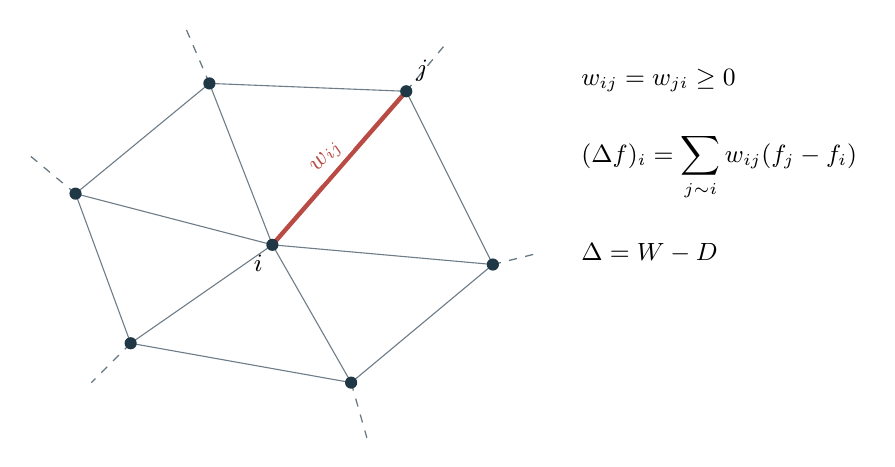
\begin{tikzpicture}[x=1cm,y=1cm]
\coordinate (a) at (0,2.2);\coordinate (b) at (1.7,3.6);\coordinate (c) at (4.2,3.5);\coordinate (d) at (5.3,1.3);\coordinate (e) at (3.5,-.2);\coordinate (f) at (.7,.3);\coordinate (i) at (2.5,1.55);
\foreach \u/\v in {a/b,b/c,c/d,d/e,e/f,f/a,a/i,b/i,c/i,d/i,e/i,f/i} {\draw[ink!65] (\u)--(\v);}
\foreach \u/\dx/\dy in {a/-.6/.5,b/-.3/.7,c/.5/.6,d/.6/.15,e/.2/-.7,f/-.5/-.5} {\draw[guide] (\u)--++(\dx,\dy);}
\draw[signalred,line width=1.6pt] (i)--node[midway,above,sloped,fill=white,inner sep=2pt] {$w_{ij}$}(c);
\foreach \u in {a,b,c,d,e,f,i} {\fill[ink] (\u) circle(2.2pt);}
\node[below left] at (i) {$i$};\node[above right] at (c) {$j$};
\node[anchor=west,align=left] at (6.3,2.55) {$w_{ij}=w_{ji}\ge0$\\[5mm]$\displaystyle(\Delta f)_i=\sum_{j\sim i}w_{ij}(f_j-f_i)$\\[5mm]$\Delta=W-D$};
\end{tikzpicture}
\end{document}
